\documentclass{article}

\usepackage[margin=1in]{geometry}
\usepackage{amsmath,amsthm,amssymb}
\usepackage{bbm, enumerate}
\usepackage{bbm, tikz}

\newenvironment{problem}[2][Problem]{\begin{trivlist}
\item[\hskip \labelsep {\bfseries #1}\hskip \labelsep {\bfseries #2.}]}{\end{trivlist}}
\newenvironment{note}[1][Note.]{\begin{trivlist}
\item[\hskip \labelsep {\bfseries #1}]}{\end{trivlist}}
\newenvironment{example}[1][Example.]{\begin{trivlist}
\item[\hskip \labelsep {\bfseries #1}]}{\end{trivlist}}

\begin{document}

\title{Matrix Analysis: Main ideas}
\author{Peter Kagey}

\maketitle

\section{Definitions}
\subsection{$M^\lambda$}
  Define $M^\lambda$ to be the complex vector space with basis the tabloids
  $\{T\}$ of shape $\lambda$.
  \begin{example}
    When $\lambda = (3, 2)$, the basis of $M^\lambda$ is \[
      \left\{
      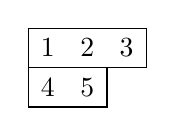
\begin{tikzpicture}[scale=0.5, baseline=-0.5ex]
        \draw (0,0) rectangle (3,1);
        \draw (0,-1) rectangle (2,0);
        \node at (0.5,0.5) {1};
        \node at (1.5,0.5) {2};
        \node at (2.5,0.5) {3};
        \node at (0.5,-0.5) {4};
        \node at (1.5,-0.5) {5};
      \end{tikzpicture},\,
      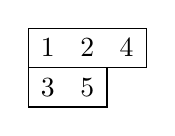
\begin{tikzpicture}[scale=0.5, baseline=-0.5ex]
        \draw (0,0) rectangle (3,1);
        \draw (0,-1) rectangle (2,0);
        \node at (0.5,0.5) {1};
        \node at (1.5,0.5) {2};
        \node at (2.5,0.5) {4};
        \node at (0.5,-0.5) {3};
        \node at (1.5,-0.5) {5};
      \end{tikzpicture},\,
      \cdots,
      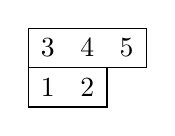
\begin{tikzpicture}[scale=0.5, baseline=-0.5ex]
        \draw (0,0) rectangle (3,1);
        \draw (0,-1) rectangle (2,0);
        \node at (0.5,0.5) {3};
        \node at (1.5,0.5) {4};
        \node at (2.5,0.5) {5};
        \node at (0.5,-0.5) {1};
        \node at (1.5,-0.5) {2};
      \end{tikzpicture}
      \right\}
    \]
  \end{example}
  \subsection{$v_T$}
    For each numbering $T$ of shape $\lambda$, there is an element
    $v_T \in M^\lambda$ given by \[
      v_T = \sum_{q \in C(T)} \operatorname{sgn}(q)\{q \cdot T\}
    \] where $C(T)$ is the column group of $T$: the set of permutations which
    preserve the columns of $T$.
  \subsection{Specht module}
    The Specht modules, denoted $S^\lambda$ is the subspace of $M^\lambda$
    given by $\operatorname{span}\{v_T : T \text{ is shape } \lambda\}$.

\end{document}